\documentclass{article}
\usepackage[margin=1in]{geometry}
\usepackage{amsmath,amsthm,amssymb}
\usepackage{bbm,enumerate,mathtools}
\usepackage{tikz,pgfplots}
\usepackage{chessboard}
\usepackage[hidelinks]{hyperref}
\usepackage{multicol} % Problem 35

\newenvironment{question}{\begin{trivlist}\item[\textbf{Question.}]}{\end{trivlist}}
\newenvironment{note}{\begin{trivlist}\item[\textbf{Note.}]}{\end{trivlist}}
\newenvironment{references}{\begin{trivlist}\item[\textbf{References.}]}{\end{trivlist}}
\newenvironment{related}{\begin{trivlist}\item[\textbf{Related.}]\end{trivlist}\begin{enumerate}}{\end{enumerate}}


\begin{document}

\rating{3}{2}
In the grid $\mathbb Z^2$, the only regular polygons that you can draw are
squares. In $\mathbb Z^3$, you can draw equilateral triangles, squares, and
regular hexagons, but no other regular polygons.

In $\mathbb Z^3$, you can also draw regular tetrahedra, cubes, and octahedra(?),
but not dodecahedra or icosahedra. (Otherwise you could draw pentagons too!)
\begin{figure}[ht!]
  \centering
  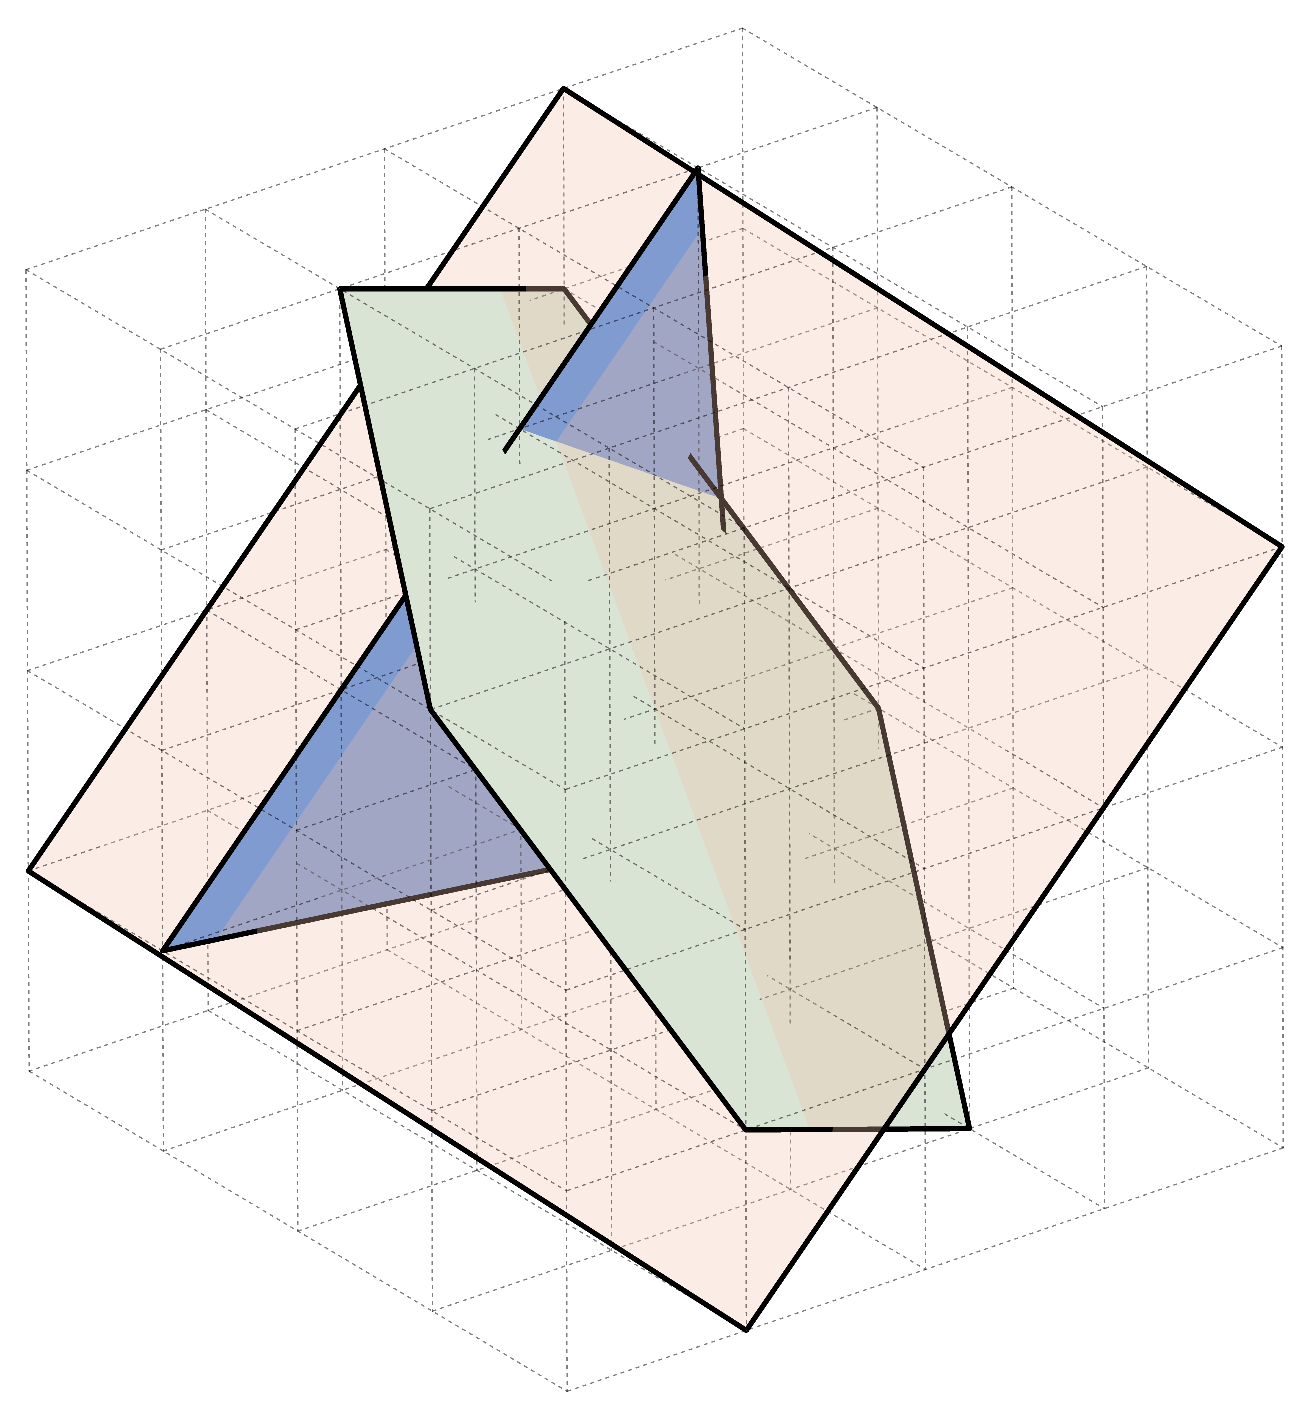
\includegraphics[scale=0.18]{assets/116_problem/polygons_in_grid_3.png}
  \caption{
    An example of an equilateral triangle, a square, and a regular hexagon
    drawn with integer coordinates in $[5]^3$.
  }
\end{figure}

\begin{question}
  How many regular $k$-dimensional polytopes can be drawn with vertices in $[n]^\ell$?
\end{question}

\begin{related}
  \item What is the asymptotic growth of the number of $k$-dimensional polytopes?
  \item What if other sorts of polytopes are considered? (E.g. Archimedean solids.)
\end{related}

\begin{references}
  \item Problems 21, 54, 66, 94, 104.
  \item A338323
\end{references}
\end{document}

% Mathematica code:
% ----------------------------------------------------------------------------
% Points := Table[Point[{x, y, z}], {x, 0, 4}, {y, 0, 4}, {z, 0, 4}];
% GridLinez := Flatten[
%   Table[
%    {Line[{{x, 0, z}, {x, 4, z}}], Line[{{0, y, z}, {4, y, z}}],
%     Line[{{x, y, 0}, {x, y, 4}}]},
%    {x, 0, 4},
%    {y, 0, 4},
%    {z, 0, 4}
%    ]
%   ]
% (*Export[
% "triangle_and_hexagon.png",
% *)
% CubeFrame[t_] := Graphics3D[
%    {PointSize[0.005], Dashed, Thickness[0.001],
%      EdgeForm[Thickness[0.004]]}
%     ~Join~
%     {Opacity[0.5]}
%     ~Join~
%     GridLinez
%     ~Join~
%     {Opacity[1]}
%     ~Join~
%     {
%      Polygon[{{1, 1, 0}, {0, 3, 1}, {1, 4, 3}, {3, 3, 4}, {4, 1,
%         3}, {3, 0, 1}}],
%      Polygon[{{1, 0, 1}, {0, 4, 0}, {4, 3, 1}}],
%      Opacity[0.3],
%      Polygon[{{1, 0, 0}, {4, 3, 0}, {3, 4, 4}, {0, 1, 4}}]
%      }
%    (*~Join~
%    {Opacity[1]}
%    ~Join~
%    Points*),
%    ViewPoint -> (Cos[t]*{180, -150, 240} +
%       Sin[t]*{-268.1, 0.9, 201.6}),
%    ViewVertical -> {0.2, -0.94, 0.27},
%    Boxed -> False,
%    SphericalRegion -> True
%    ];(*,
% ImageSize \[Rule] 2000]*)
